% Entrega 2: Integración de los límites de municipios PDET
% Compilar desde docs/delivery2/:  latexmk -pdf entrega2.tex
% Cada integrante escribe su parte en secciones/<tramo>.tex para no pisar a los demás.
\documentclass[11pt,a4paper]{article}

\usepackage[T1]{fontenc}
\usepackage[utf8]{inputenc}
\usepackage[spanish,es-noshorthands,es-tabla]{babel}
\usepackage{lmodern}
\usepackage[left=2.3cm,right=2.3cm,top=2.2cm,bottom=2.4cm]{geometry}
\usepackage{graphicx}
\usepackage{booktabs}
\usepackage{float}
\usepackage{tabularx}
\usepackage{array}
\usepackage{xcolor}
\usepackage{enumitem}
\usepackage[font=small,labelfont=bf]{caption}
\usepackage{fancyhdr}
\usepackage[hidelinks]{hyperref}

\definecolor{acento}{HTML}{1F5FAF}
\newcommand{\brkus}{\textunderscore\allowbreak}
\newcommand{\f}[1]{{\ttfamily\let\_\brkus #1}}
\newcommand{\pendiente}[1]{\par\fbox{\parbox{\dimexpr\textwidth-2\fboxsep-2\fboxrule}{\small\color{gray}Pendiente: #1}}\par}
\newcolumntype{L}{>{\raggedright\arraybackslash}X}
\setlist{nosep,leftmargin=1.4em}
\setlength{\parskip}{0.45em}
\setlength{\parindent}{0pt}
\renewcommand{\arraystretch}{1.15}

\pagestyle{fancy}
\fancyhf{}
\lhead{\small Proyecto final DBA · Entrega 2}
\rhead{\small Techos solares en municipios PDET}
\cfoot{\small \thepage}
\renewcommand{\headrulewidth}{0.3pt}

\begin{document}

\begin{center}
  {\small Pontificia Universidad Javeriana · Administración de Bases de Datos · 2026-30}\\[0.9em]
  {\LARGE\bfseries\color{acento} Entrega 2: Integración de los límites\\[0.2em] de municipios PDET}\\[0.8em]
  {\large Potencial solar en techos de los municipios PDET (UPME)}\\[0.8em]
  Derek Sarmiento · José Medina · Miguel Duarte · Sebastián Sánchez Vásquez · Samuel Emperador\\[0.3em]
  {\small Prof. Andrés Oswaldo Calderón Romero, Ph.D. · Lunes 9 de noviembre de 2026}\\[0.3em]
  {\small Repositorio: \url{https://github.com/dba-upme-pdet/techos-solares-pdet}}
\end{center}

\section{Objetivo y flujo}

Esta entrega integra los límites oficiales de los 170 municipios PDET en MongoDB: se descarga la capa municipal del Marco Geoestadístico Nacional (MGN 2025) del DANE, se valida contra la lista oficial de municipios PDET, se convierte a documentos GeoJSON compatibles con el esquema de la Entrega 1, se carga en la colección \f{municipalities} y se verifica el índice \f{2dsphere}.

Los scripts comparten un contrato (\f{scripts/entrega2\_contracts.py}, versión \f{entrega2-mgn-v1}): nombres de campos, CRS, regla de códigos DIVIPOLA y formato de los reportes en \f{outputs/}. El cruce entre el MGN y la lista PDET es siempre por código DIVIPOLA de 5 dígitos, nunca por nombre.

\begin{table}[H]
\centering\small
\caption{Pasos de la Entrega 2, en orden de ejecución.}
\begin{tabularx}{\textwidth}{@{}>{\raggedright\arraybackslash}p{4.4cm} p{3.4cm} L@{}}
\toprule
Script & Responsable & Entrada $\rightarrow$ salida \\
\midrule
\f{01\_download\_mgn.py} & Derek Sarmiento & WFS MGN 2025 $\rightarrow$ capa GeoPackage y \f{mgn\_download\_manifest.json} \\
\f{01\_validate\_mgn.py} & Samuel Emperador & capa + \f{MunicipiosPDET.xlsx} $\rightarrow$ \f{mgn\_validation\_report.json}, resumen y cruce CSV \\
\f{02\_prepare\_municipalities.py} & José Medina & capa + Excel $\rightarrow$ \f{municipalities.geojsonl} (170 documentos) \\
\f{02\_load\_municipalities.py} & Miguel Duarte & GeoJSONL $\rightarrow$ colección \f{municipalities} \\
\f{02\_verify\_spatial.py} & Sebastián Sánchez & colección $\rightarrow$ \f{explain()} sobre \f{geometry\_2dsphere} \\
\bottomrule
\end{tabularx}
\end{table}

% Derek Sarmiento (scripts/01\_download\_mgn.py)
% Redactada por Miguel Duarte a partir del script, su self-check, el recibo y la
% corrida del 9 de noviembre de 2026; pendiente de revisión de Derek.
\section{Descarga del Marco Geoestadístico Nacional}\label{sec:descarga}

\textit{Responsable: Derek Sarmiento. Script: \f{scripts/01\_download\_mgn.py}.}

\subsection{Objetivo}

Obtener la capa municipal completa del MGN 2025 del DANE (1122 municipios), con los campos que usa el diccionario de datos de la Entrega~1 (\f{MPIO\_CDPMP}, \f{MPIO\_CNMBR}, \f{MPIO\_NAREA}, \f{DPTO\_CCDGO}), dejarla como un GeoPackage legible y acompañarla de un manifiesto que diga de dónde salieron los bytes y si la descarga es nacional y verificable.

\subsection{Fuente}

La fuente es el servicio WFS~2.0 público del DANE, capa \f{Serv\_CapasMGN\_2025:Municipio}, el acceso OGC que publica la ficha \f{8xdp-fsgm} de \f{datos.gov.co}. Se pide en GML~3.2 con \f{srsName=urn:ogc:def:crs:EPSG::4686}, en seis páginas de 200 registros (\f{startIndex} 0, 200, 400, 600, 800 y 1000). La página renderizada del geoportal y el \f{FeatureServer} REST no se usan: el cortafuegos del DANE los bloquea para clientes automáticos. La verificación TLS queda siempre activa.

\subsection{Entradas y salidas}

\begin{table}[H]
\centering\small
\caption{Contrato de entrada y salida de \f{01\_download\_mgn.py}.}
\begin{tabularx}{\textwidth}{@{}p{5.6cm} p{2.2cm} L@{}}
\toprule
Pieza & Rol & Condición \\
\midrule
\f{config.yaml} (\f{sources.mgn.wfs}) & entrada & servicio, \f{typeName}, \f{srsName}, plan de páginas y \f{expected\_feature\_count = 1122} \\
\f{outputs/mgn\_wfs\_source\_receipt.json} & entrada & por página: URL, bytes, \f{sha256}, \f{content\_sha256} y \f{server\_timestamp} \\
\f{data/raw/mgn2025/wfs/page\_XXXX.gml} & salida & respuestas del WFS guardadas byte a byte (fuera de Git) \\
\f{data/raw/mgn2025/wfs/municipio.gpkg} & salida & 1122 municipios, EPSG:4686, longitud/latitud (fuera de Git) \\
\f{outputs/mgn\_download\_manifest.json} & salida & \f{status = complete}, \f{claims\_national\_download = true}, SHA256 de la capa y coincidencia de cada página \\
\bottomrule
\end{tabularx}
\end{table}

\subsection{Método}

\begin{enumerate}
  \item \textbf{Plan oficial.} El recibo solo cuenta si su servicio, \f{typeName}, \f{srsName}, URLs, \f{startIndex} y \f{number\_matched} son los de \f{config.yaml}. Un recibo de otro tamaño, aunque sus bytes coincidan, no habilita una descarga nacional.
  \item \textbf{Caché o descarga.} Si las seis páginas locales coinciden con el recibo, no se contacta el servidor. Si no, se hace un intento por página y la corrida se detiene al primer fallo de red o TLS. Una respuesta que no coincide con el recibo se rechaza.
  \item \textbf{Coincidencia por bytes o por contenido.} El WFS escribe en el elemento raíz un atributo \f{timeStamp} con la hora de cada respuesta, así que dos descargas del mismo contenido nunca tienen el mismo SHA256. Por eso el recibo guarda además \f{content\_sha256}: el SHA256 de la página con el valor de ese único atributo vaciado. Una página vale si coincide por bytes o por contenido; los archivos descargados no se modifican.
  \item \textbf{Lectura del GML.} Los elementos vienen con alias en español y se mapean de forma explícita (\f{Código\_DANE\_concatenado\_departamento\_y\_municipio} $\rightarrow$ \f{MPIO\_CDPMP}, \f{Nombre\_municipio} $\rightarrow$ \f{MPIO\_CNMBR}, \f{Área\_departamento\_en\_kilómetros\_cuadrados} $\rightarrow$ \f{MPIO\_NAREA}, entre otros). Cada \f{posList} viene en latitud/longitud, como declara EPSG:4686, y se guarda en longitud/latitud.
  \item \textbf{Controles de la capa.} Exactamente 1122 registros, igual a \f{numberMatched}; códigos de 5 dígitos sin repetidos; un único \f{srsName} en todas las páginas.
  \item \textbf{Unidad del área.} El nombre del elemento dice kilómetros cuadrados; además se compara \f{MPIO\_NAREA} con el área geodésica WGS84 de cada contorno. Si la mediana del cociente no cae entre 0,5 y 2, no se declara la unidad y la descarga no queda como nacional.
  \item \textbf{Manifiesto honesto.} Si algo falla, el manifiesto actual queda en \f{blocked} o \f{invalid} con \f{claims\_national\_download = false}, y un manifiesto exitoso anterior se conserva aparte en \f{mgn\_download\_manifest.history.json}. Si la capa y los hash no cambiaron, la siguiente corrida solo la revalida.
\end{enumerate}

\subsection{Pruebas}

\f{python scripts/01\_download\_mgn.py --self-check} usa fixtures etiquetados y nunca cuenta como descarga del DANE. Resultado: \textbf{22/22 OK}. Cubre la elección del ZIP correcto en el HTML del geoportal, la lectura de la unidad desde metadatos, el rechazo de CRS ausente o distinto, de capas sin \f{MPIO\_NAREA} o ilegibles, la inversión de ejes del GML, que un recibo de un municipio no se anuncie como nacional, que un fallo TLS no deje el manifiesto anterior como actual, y los ocho casos del hash de contenido: coincidencia por bytes y por contenido, rechazo de un byte distinto fuera del \f{timeStamp}, rechazo sin \f{content\_sha256}, rechazo de dos \f{timeStamp} en la raíz, reconstrucción del SHA256 original y el \f{--backfill-receipt} aceptado y rechazado.

\subsection{Resultados}

Las respuestas originales se obtuvieron el 8 de noviembre de 2026 entre las 15:23 y las 15:24 (hora de Bogotá), en 6,4 a 8,5~s por página. En la noche del 8 de noviembre (21:38, hora de Bogotá) se volvieron a descargar las seis páginas: tienen el mismo tamaño y, con el \f{timeStamp} original reinsertado, reproducen exactamente el SHA256 del recibo. Es decir, son el mismo contenido; solo cambió la hora que escribe el servidor.

\begin{table}[H]
\centering\small
\caption{Páginas del recibo (\f{mgn\_wfs\_source\_receipt.json}).}
\begin{tabular}{@{}lrlll@{}}
\toprule
Página & Bytes & \f{sha256} & \f{content\_sha256} & \f{timeStamp} original \\
\midrule
\f{page\_0000.gml} & 26\,416\,139 & \f{5d600d25b928\ldots} & \f{ce7a0d0ca809\ldots} & 20:23:33Z \\
\f{page\_0200.gml} & 22\,174\,892 & \f{6900fa419817\ldots} & \f{09b5856d94dd\ldots} & 20:23:40Z \\
\f{page\_0400.gml} & 25\,069\,453 & \f{168772c3d7bd\ldots} & \f{89e051c376c9\ldots} & 20:23:47Z \\
\f{page\_0600.gml} & 29\,395\,276 & \f{d6b3ee0b193b\ldots} & \f{0c271831db52\ldots} & 20:23:54Z \\
\f{page\_0800.gml} & 21\,884\,852 & \f{2b8496abd8a2\ldots} & \f{31f8cfda05d0\ldots} & 20:24:02Z \\
\f{page\_1000.gml} & 27\,119\,583 & \f{2eadfebad833\ldots} & \f{11a39ac93152\ldots} & 20:24:09Z \\
\bottomrule
\end{tabular}
\end{table}

\begin{table}[H]
\centering\small
\caption{Capa resultante según \f{mgn\_download\_manifest.json}.}
\begin{tabularx}{\textwidth}{@{}p{5.6cm} L@{}}
\toprule
Indicador & Valor \\
\midrule
Estado & \f{complete}, \f{national\_complete = true}, \f{claims\_national\_download = true} \\
Registros & 1122 (igual a \f{numberMatched}), 0 geometrías nulas, todas \f{MultiPolygon} \\
Año de versión DANE & 954 municipios de 2024 y 168 de 2025 (no se filtra) \\
CRS & EPSG:4686 declarado por el WFS; coordenadas guardadas en longitud/latitud \\
Unidad de \f{MPIO\_NAREA} & km$^2$; cociente atributo/área geodésica: mediana 0,9994, mínimo 0,9984, máximo 1,0209 \\
Capa & \f{municipio.gpkg}, 100,6~MB \\
Coincidencia con el recibo & 6/6 páginas por contenido (descarga del 8 de noviembre, 21:38) \\
\bottomrule
\end{tabularx}
\end{table}

El SHA256 del GeoPackage cambia en cada escritura porque el formato guarda metadatos propios; el manifiesto registra el de la corrida actual y la preparación lo comprueba. Lo que se mantiene estable es el producto: a partir de estas páginas, la preparación produce siempre el mismo GeoJSONL (sección~\ref{sec:preparacion}).

\subsection{Limitaciones}

\begin{itemize}
  \item No se descargó el ZIP oficial del MGN ni su \f{.prj}, así que el CRS del archivo original no está probado (\f{original\_archive\_crs\_proven = false}). Se usa el \f{srsName} que declara el WFS; el almacenamiento REST del mismo servicio informa EPSG:3857.
  \item El elemento del área se llama \emph{Área\_departamento} aunque el objeto es un municipio; la unidad se confirma con el cociente geodésico, no con el nombre solo.
  \item Las páginas GML y el GeoPackage están fuera de Git por tamaño (unos 150~MB). Para reproducir la cadena basta con volver a descargarlas: el hash de contenido las valida contra el recibo.
\end{itemize}

% Samuel Emperador: filtrado y validación de municipios PDET (scripts/01_validate_mgn.py)
\section{Filtrado y validación de municipios PDET}\label{sec:validacion}

\textit{Responsable: Samuel Emperador. Script: \path{scripts/01_validate_mgn.py}.}

\subsection{Objetivo}

Antes de preparar y cargar los municipios hay que comprobar que la capa del MGN y la lista oficial PDET son coherentes entre sí: que cada uno de los 170 municipios PDET existe en el MGN con un código DIVIPOLA correcto, que ningún código está repetido y que las geometrías sirven para MongoDB. El script solo verifica y reporta; no modifica la capa ni repara geometrías (eso lo hace \path{02_prepare_municipalities.py}).

\subsection{Método}

\begin{enumerate}
  \item Lee el manifiesto de la descarga y se detiene (salida 2) si no acredita la capa nacional: sin manifiesto, \f{status} distinto de \f{complete}, capa ausente o SHA256 distinto del declarado.
  \item Lee la capa (GeoPackage, EPSG:4686) y la hoja \f{Hoja1} de \f{MunicipiosPDET.xlsx}.
  \item Normaliza los códigos con \f{zfill\_digits} del contrato: \f{MPIO\_CDPMP} y \f{Código DANE Municipio} a 5 dígitos (5031 $\rightarrow$ 05031), \f{DPTO\_CCDGO} a 2.
  \item Revisa la capa, la lista y el cruce por código (tabla~\ref{tab:verificaciones}). Cada geometría se clasifica como nula, vacía, no poligonal o inválida; para las inválidas se guarda el motivo de \f{shapely.explain\_validity}.
  \item Compara los nombres solo como información, separando las diferencias que son únicamente de tildes.
  \item Escribe tres salidas en \path{outputs/}: \f{mgn\_validation\_report.json} (resultado de cada verificación y \f{status} \f{valid}, \f{invalid} o \f{blocked\_no\_layer}), \f{mgn\_validation\_summary.md} y \f{pdet\_mgn\_crosswalk.csv} (una fila por municipio PDET).
\end{enumerate}

Una verificación es \emph{bloqueante} si su falla impide cargar los municipios. Las geometrías inválidas fuera de los PDET y las diferencias de nombre solo generan aviso. El código de salida es 0 si todas las bloqueantes pasan y 1 si alguna falla, así que los scripts siguientes (o quien los corra) pueden leer \f{status} antes de preparar o cargar.

\subsection{Resultados}

El reporte vigente fue generado por Miguel el 9 de noviembre de 2026 a las 07:27:37 (hora de Bogotá) sobre la capa de 1122 municipios que produce \path{01_download_mgn.py}. Reproduce el resultado inicial documentado por Samuel el 8 de noviembre: \textbf{\f{valid}}, 19 de 20 verificaciones en OK y un aviso informativo.

\begin{table}[htbp]
\centering\small
\caption{Verificaciones de \protect\path{01_validate_mgn.py} sobre la capa real. B: bloqueante.}\label{tab:verificaciones}
\begin{tabularx}{\textwidth}{@{}r L c l@{}}
\toprule
\# & Verificación & B & Resultado \\
\midrule
1 & Campos obligatorios del MGN (\f{MPIO\_CDPMP}, \f{MPIO\_CNMBR}, \f{MPIO\_NAREA}, \f{DPTO\_CCDGO}) & sí & OK \\
2 & Capa nacional con 1122 municipios & sí & OK: 1122 \\
3 & CRS EPSG:4686 & sí & OK \\
4 & \f{MPIO\_CDPMP} es DIVIPOLA de 5 dígitos & sí & OK: 0 errores \\
5 & Prefijo de \f{MPIO\_CDPMP} = \f{DPTO\_CCDGO} & sí & OK: 0 errores \\
6 & Sufijo de \f{MPIO\_CDPMP} = \f{MPIO\_CCDGO} & sí & OK: 0 errores \\
7 & Sin códigos repetidos en el MGN & sí & OK: 0 \\
8 & \f{MPIO\_NAREA} numérica y positiva & sí & OK \\
9 & Geometrías válidas en el MGN & no & OK: 0 inválidas \\
10 & Vértices dentro de la ventana lon/lat de Colombia & sí & OK \\
11 & Lista PDET con 170 filas & sí & OK: 170 \\
12 & Códigos PDET numéricos & sí & OK \\
13 & Sin códigos repetidos en la lista PDET & sí & OK: 0 \\
14 & 16 subregiones PDET & sí & OK: 16 \\
15 & Prefijo del código PDET = departamento del Excel & sí & OK \\
16 & Todos los municipios PDET están en el MGN & sí & OK: 0 faltantes \\
17 & Departamento del Excel = \f{DPTO\_CCDGO} del MGN & sí & OK: 0 \\
18 & Geometrías de los 170 PDET válidas & sí & OK: 0 inválidas \\
19 & Nombres iguales entre Excel y MGN & no & Aviso: 15 distintos \\
20 & Cruce completo de 170 municipios PDET & sí & OK: 170 \\
\bottomrule
\end{tabularx}
\end{table}

Los 170 municipios PDET cruzan con el MGN: no falta ninguno, no hay códigos repetidos en ninguna de las dos fuentes y los departamentos coinciden. Las 1122 geometrías son \f{MultiPolygon} válidas, ninguna nula o vacía, y todas caen en la ventana de Colombia (un control para detectar ejes latitud/longitud invertidos, sin certificar por sí solo el CRS). El área MGN de los 170 municipios suma 389\,182~km\textsuperscript{2}. La figura~\ref{fig:mapa-pdet} muestra el resultado del cruce.

\begin{figure}[htbp]
\centering
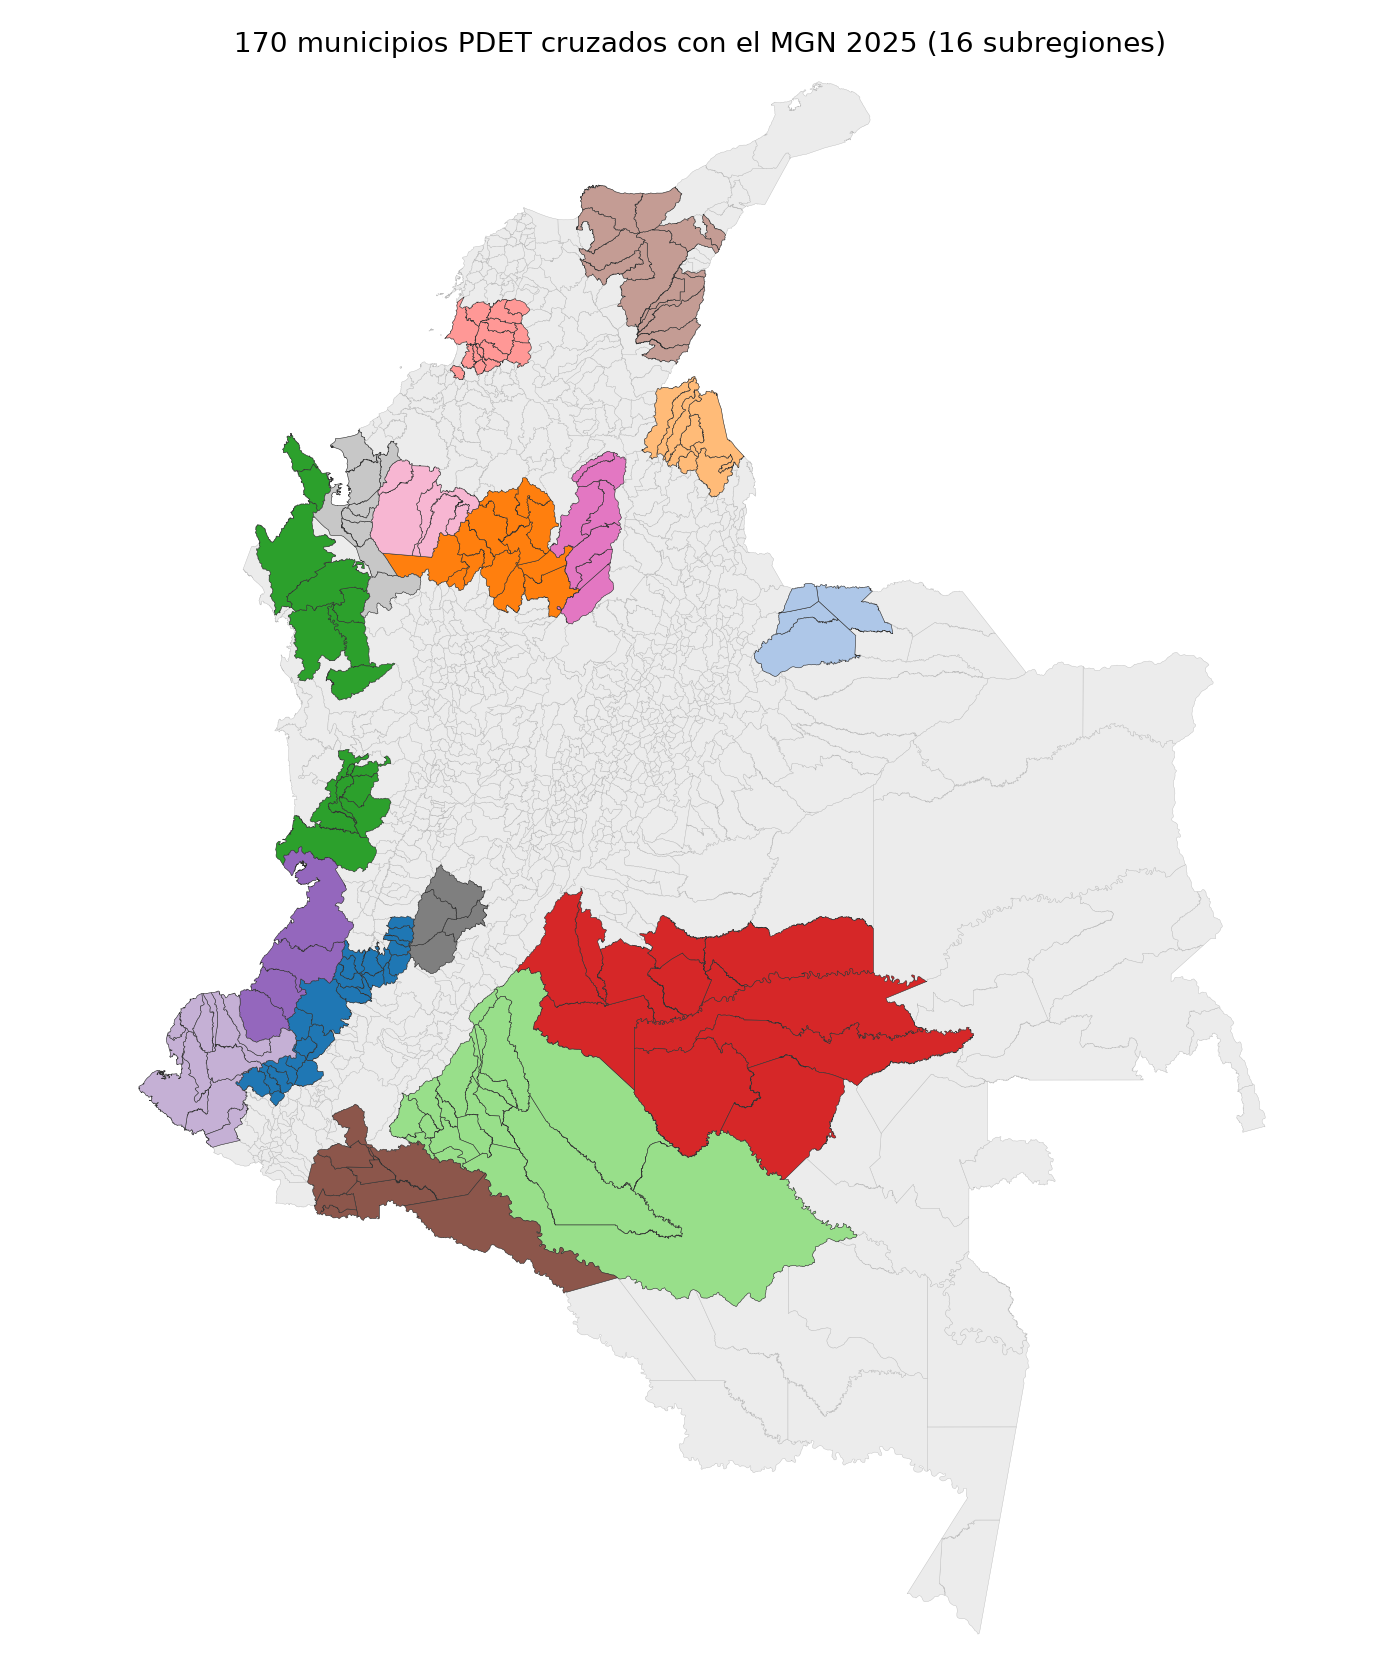
\includegraphics[width=0.62\textwidth]{figuras/mapa_pdet_validacion.png}
\caption{Municipios PDET cruzados con la capa MGN 2025; el color distingue la subregión. Generado con \protect\path{docs/delivery2/figuras/build_mapa_pdet.py} a partir de \f{pdet\_mgn\_crosswalk.csv}.}\label{fig:mapa-pdet}
\end{figure}

El único aviso son 15 nombres escritos distinto en el Excel y en el MGN (tabla~\ref{tab:nombres}): 9 difieren solo en tildes y 6 usan otra forma oficial del nombre. Ninguno afecta el cruce, que es por código, y la cifra coincide con \f{name\_mismatches} del reporte de preparación. Los documentos de \f{municipalities} usan el nombre del MGN.

\begin{table}[htbp]
\centering\small
\caption{Nombres distintos entre \f{MunicipiosPDET.xlsx} y el MGN 2025.}\label{tab:nombres}
\begin{tabularx}{\textwidth}{@{}l L L l@{}}
\toprule
Código & Excel & MGN & Tipo \\
\midrule
19548 & PIENDAMÓ & PIENDAMÓ - TUNÍA & forma oficial \\
50711 & VISTA HERMOSA & VISTAHERMOSA & forma oficial \\
70523 & SAN ANTONIO DE PALMITO & PALMITO & forma oficial \\
70823 & TOLÚ VIEJO & SAN JOSÉ DE TOLUVIEJO & forma oficial \\
19418 & LÓPEZ & LÓPEZ DE MICAY & forma oficial \\
86573 & LEGUÍZAMO & PUERTO LEGUÍZAMO & forma oficial \\
19821 & TORIBIO & TORIBÍO & tildes \\
27099 & BOJAYA & BOJAYÁ & tildes \\
27150 & CARMEN DEL DARIEN & CARMEN DEL DARIÉN & tildes \\
18256 & EL PAUJIL & EL PAUJÍL & tildes \\
70204 & COLOSO & COLOSÓ & tildes \\
52427 & MAGÜI & MAGÜÍ & tildes \\
52835 & SAN ANDRES DE TUMACO & SAN ANDRÉS DE TUMACO & tildes \\
23682 & SAN JOSE DE URE & SAN JOSÉ DE URÉ & tildes \\
05665 & SAN PEDRO DE URABA & SAN PEDRO DE URABÁ & tildes \\
\bottomrule
\end{tabularx}
\end{table}

\subsection{Pruebas del validador}

Como la capa real no tiene errores, cada verificación se probó también con figuras sintéticas (\f{python} \path{scripts/01_validate_mgn.py} \f{--self-check}, 19/19): municipio PDET ausente del MGN, código repetido en cada fuente, prefijo de departamento distinto, código no numérico, polígono autointersecado (falla dentro de los PDET y solo avisa fuera de ellos), punto en lugar de polígono, ejes invertidos, CRS EPSG:3857, capa incompleta, campo obligatorio faltante, y manifiesto ausente o bloqueado (salida 2).

\subsection{Observaciones}

\begin{itemize}
  \item El cambio de \f{timeStamp} que bloqueaba la comparación binaria ya se resuelve mediante \f{content\_sha256}, conservando los bytes originales. El manifiesto vigente registra coincidencia por contenido de las seis páginas (sección~\ref{sec:descarga}).
  \item El SHA256 del GeoPackage puede cambiar entre escrituras por sus metadatos; el GeoJSONL preparado sí sale idéntico. Por eso el validador compara la capa con el manifiesto de la misma corrida.
\end{itemize}

% José Medina (scripts/02\_prepare\_municipalities.py)
\section{Preparación de los documentos de municipios}

\textit{Responsable: José Medina. Script: \f{scripts/02\_prepare\_municipalities.py}.}

\pendiente{José Medina escribe esta sección en \f{docs/delivery2/secciones/preparacion.tex}.}

% Miguel Duarte (scripts/02\_load\_municipalities.py)
\section{Carga en MongoDB}

\textit{Responsable: Miguel Duarte. Script: \f{scripts/02\_load\_municipalities.py}.}

\pendiente{Miguel Duarte escribe esta sección en \f{docs/delivery2/secciones/carga.tex}.}

% Sebastián Sánchez Vásquez (scripts/02\_verify\_spatial.py)
\section{Verificación del índice espacial}

\textit{Responsable: Sebastián Sánchez Vásquez. Script: \f{scripts/02\_verify\_spatial.py}.}

\pendiente{Sebastián Sánchez Vásquez escribe esta sección en \f{docs/delivery2/secciones/verificacion.tex}.}


\end{document}
